%!TEX root = ./report.tex
\section{Solution}
\label{sec:solution}
Our prototype combines several open source technologies to attain an extensible solution with two reusable MWE2 client side workflows at its core. The setup allows the user to edit a subset of IFC in an auto-generated Eclipse editor in between the two workflows. The two building models are stored on a BIMServer for possible merging, version control, and collaboration through the client-server design pattern, as this section will explain further. The prototype serves as an open source alternative to similar, proprietary BIM software.

\subsection{IFC Meta Model}
% Our meta model is generated from ifcXML XSD, only handles ifcXML
% BIMServer - tightly coupled, but handles .ifc. Handles references as string
% Jim Steel model. Seems to be better, but we have no deserializer.
\label{subsec:ifc_meta_model}
The prototype uses an IFC meta model that is auto-generated from the XML Schema Definition (XSD) of ifcXML.\footnote{ifcXML XSD: \url{http://buildingsmart-tech.org/ifcXML/IFC2x3/FINAL/IFC2X3.xsd}} This allows utilisation of the XML serialiser and deserialiser provided by EMF to convert ifcXML to and from its Java representation.  One of the advantages of using these tools is that we do not have to develop any serialisers ourselves. However, generating the meta model from an XSD also means that the client application of the prototype only supports ifcXML, and not  the more widely used IFC-EXPRESS format. Because BIMServer accepts and generates both formats, this is a minor concern. But it means that the client side of the prototype relies on BIMServer for IFC-EXPRESS handling.

Although we chose not to use it, BIMServer also provides a meta model for IFC. This meta model comes with a custom serialiser and deserialiser for IFC-EXPRESS. We found that using this model and the provided serialisation tools was undesirable, as it would mean that the client application of the prototype would be completely dependent on the BIMServer. An advantage of using this meta model would be that it resembles the documented IFC specification more closely than the auto-generated meta model (even though both are equally correct). Specifically, the BIMServer meta model models inverse relationships, which are not represented as intuitively in the auto-generated meta model.

A third meta model for IFC has been created by Jim Steel, Lecturer at the University of Queensland.\footnote{Jim Steel at the University of Queensland: \url{http://itee.uq.edu.au/~uqjstee8/}}\footnote{Jim Steel's model can be found at \url{http://www.emn.fr/z-info/atlanmod/index.php/Ecore#ifc2x3_0.1}} This meta model seems to model all relationships better than the two aforementioned models, but does not provide a deserialiser to any IFC format. As it is not within the scope of this project to create a deserialiser for such a meta model, it was not used. However, using this meta model could be considered as a future improvement.

\subsection{Pipes DSL}
\label{subsec:pipes_dsl}

\begin{figure}[t]
    \centering
        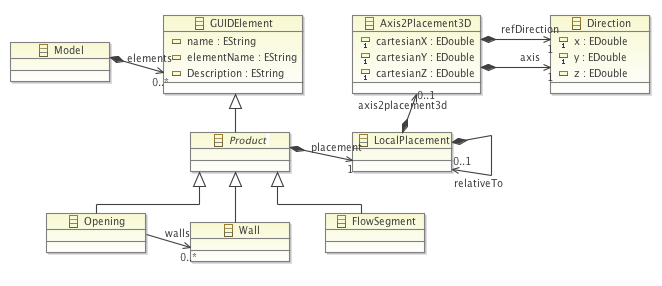
\includegraphics[width=110mm]{images/PipesEcoreModel.png}
    \caption{Pipes DSL Ecore meta model.}
    \label{fig:pipes_dsl_ecore_model}
\end{figure}

\begin{figure}[t]
    \centering
        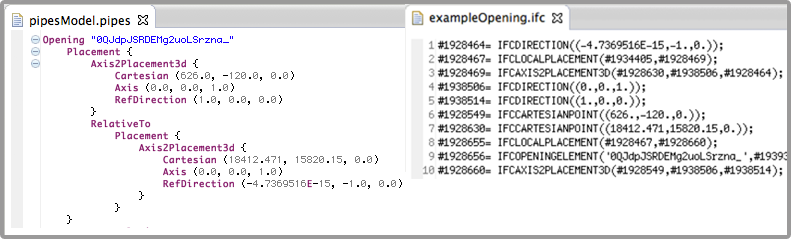
\includegraphics[width=120mm]{images/pipesAndExpressExample.png}
    \caption{A comparison of an opening specification in the Pipes DSL (left) and the IFC-EXPRESS format (right) with placement references and metadata.}
    \label{fig:pipes_express_comparison}
\end{figure}

The simple Pipes DSL serves as the front-end of the prototype. Figure \ref{fig:pipes_dsl_ecore_model} shows the Ecore model that the DSL is built upon. Compared to Figure \ref{fig:ifcheirachy}, all the critical elements of the domain are still present, but the inheritance hierarchy has been greatly simplified. As shown, Opening, Wall, and FlowSegment are top level elements, each with a physical location specified by the LocalPlacement reference. Figure \ref{fig:pipes_express_comparison} depicts an example of an opening as it is defined in the Pipes DSL in an uncluttered and manageable way, compared to the IFC-EXPRESS format. The textual syntax has been created from the Pipes DSL meta model using Xtext, which also provides an editor with syntax highlighting and autocompletion. The editor is launched as an Eclipse instance.

\subsection{BIMServer}
The overall workflow of the end product is shown in Figure \ref{fig:overall_product_workflow}. As described in J\o rgensen's workflow document\,\cite{jorgensen12}, a construction model and a plumbing model are combined into one single model that needs to be verified. So-called openings, i.e. holes in walls and floors, need to be present where the plumbing model defines pipes to be installed. The merging of these models is executed on the BIMServer by the user as the first step of the workflow. When the models have been merged, the client application can retrieve the merged model as ifcXML. The user is now allowed to edit and add elements to the subset of the model on the client side before saving the building back to the BIMServer as ifcXML.

Note that the solution does not take concurrent editing by multiple clients into account, although BIMServer does support version control and change notifications for this exact purpose.

\begin{figure}[h]
    \centering
        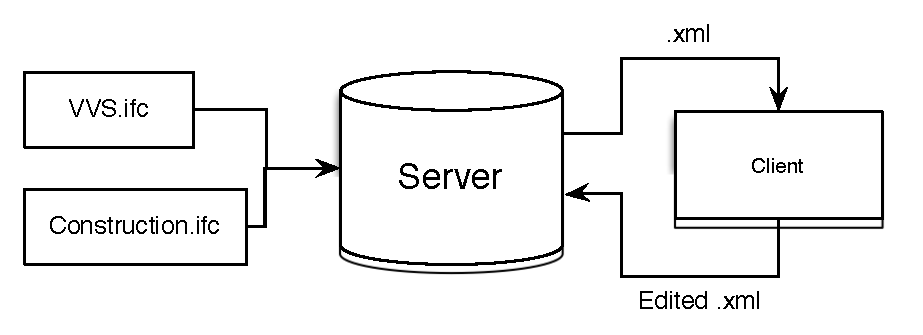
\includegraphics[width=70mm]{images/CompleteWorkflow.pdf}
    \caption{Overall product workflow starting with a merge of two models. The user can edit a subset of the model through the client-side application.}
    \label{fig:overall_product_workflow}
\end{figure}

Although many tools exist for this job, we let a BIMServer instance handle the initial merging of plumbing and construction models. An advantage of the BIMServer is that it also provides conversion tools, which allows the user to retrieve the saved building in other formats as well as a Java client library\,\cite{beetz10}.

\subsection{Client Side}
The client side of the prototype is implemented as a two MWE2 workflows, and a textual editor for the Pipes DSL. The workflows, called IFC2Pipes and Pipes2IFC, invoke a series of workflow components, implemented in Xtend. The IFC2Pipes workflow executes the transformations from IFC to the Pipes DSL, after which the textual editor can be used to modify the Pipes DSL model. When the editing is complete, the Pipes2IFC workflow is run to update the IFC model based on the changes in the Pipes DSL model.

\begin{figure}[t]
    \centering
        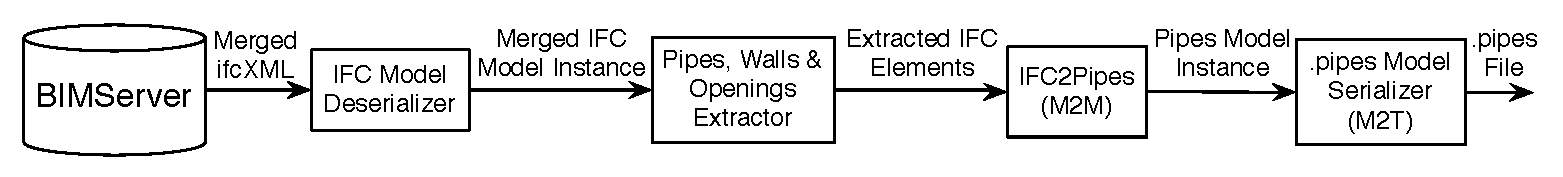
\includegraphics[width=114mm]{images/IFC2Pipes.pdf}
    \caption{IFC2Pipes workflow. Processes ifcXML from BIMServer and outputs a .pipes file, loadable in the Pipes DSL editor.}
    \label{fig:IFC2PipesWorkflow}
\end{figure}
\subsubsection{IFC2Pipes}
Figure \ref{fig:IFC2PipesWorkflow} illustrates the first workflow. The newest revision of the IFC model is downloaded from BIMServer as ifcXML, and cached on disk. This is deserialised by an auto-generated deserialiser, which was produced alongside the meta model. After the model has been loaded into memory, the relevant elements (see Section \ref{subsec:requirements}) are extracted by a workflow component, IFCExtractor. These elements are passed to the IFC2PipesTransformer component, which creates a Pipes DSL model based on the extracted elements. This is done by creating a Pipes DSL model equivalent for each extracted element, preserving the GUID. Finally, using an Xpand template, textual Pipes DSL is generated, and serialised to a file on disk.

\begin{figure}[t]
    \centering
        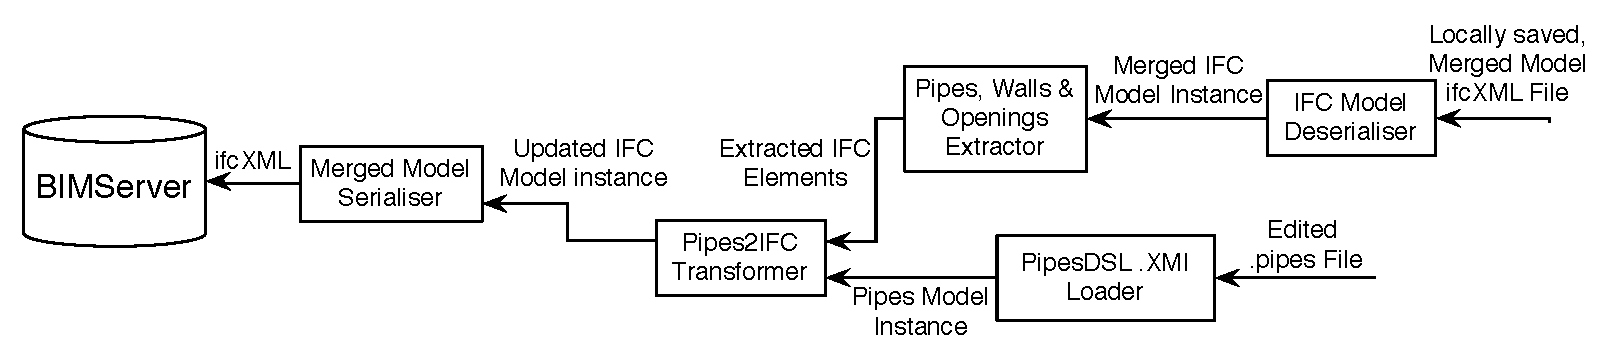
\includegraphics[width=120mm]{images/Pipes2IFC.pdf}
    \caption{Pipes2IFC workflow. Updates the main IFC model with the changes written in the Pipes DSL editor, then sends the IFC model back to BIMServer.}
    \label{fig:Pipes2IFCWorkflow}
\end{figure}
\subsubsection{Pipes2IFC}
Figure \ref{fig:Pipes2IFCWorkflow} shows the second workflow. As MWE2 workflows run in their own processes, it is necessary to deserialise the model again, this time using the cached ifcXML. Consequently, the IFCExtractor must also be invoked again. The edited Pipes DSL file is also deserialised and instantiated as a model. By comparing the two models, the Pipes2IFCTransformer updates the IFC model. To determine if an element has been added, updated, or removed, the GUIDs of the elements in the two models are used in the following way.
\begin{itemize}
\item If a GUID appears on an element in the Pipes DSL model, which does not exist in the IFC model, the element is transformed to its IFC equivalent, and added to the IFC model.
\item If a GUID exists in both models, but the elements have different metadata, the IFC element is updated.
\item If a GUID exists in the IFC model, but not in the Pipes DSL mode, it is removed from the IFC model.
\end{itemize}
When the IFC model has been appropriately updated, a simple garbage collection routine removes any orphaned elements or references, and the model is serialized as ifcXML, and sent to BIMServer as a new revision.
